\section*{1. Übung}
\subsection*{1.1. Aufgabe}
\begin{equation}
\begin{split}
	b \in \left\{ x_1 \cdot \begin{pmatrix*} 1\\ 1\\ 1 \end{pmatrix*} + x_2 \cdot \begin{pmatrix*} 1\\ -2\\ -1 \end{pmatrix*} | x_1, x_2 \in \R \right\}
\end{split}
\end{equation}
Da $b$ aber eben nicht Element dieser Menge ist, gibt es keine Lösung.
Man möchte, dass $Ax^\star$ möglichst nahe daran liegt.


eine möglichst \glqq gute\grqq{} Lösung könnte sinnvollerweise foglendes erfüllen:

\[
\norm{Ax-b}^2_2 \longrightarrow min
\]

\subsection*{1.2. Aufgabe}
\subsubsection*{1.2.a}
\begin{figure}[ht]
	\centering
	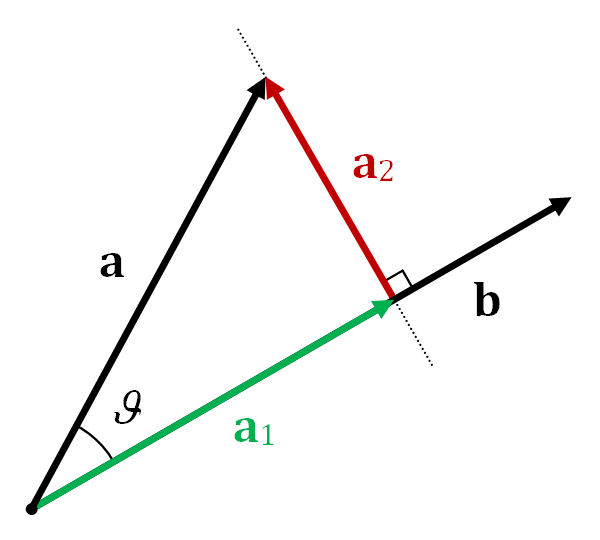
\includegraphics[scale=.3]{Projection_and_rejection.png}
\end{figure}

\begin{equation}\begin{split}
	u = \begin{pmatrix*}1\\1\\1\end{pmatrix*}\quad;\quad
	v = \begin{pmatrix*}0\\2\\1\end{pmatrix*}\\
	v = v_{\bot} + v_{\parallel}\\\\
\end{split}\end{equation}
\begin{equation}\begin{split}
	<v; u>
	&= <v_{\bot} + v_{\parallel}; u>\\
	&= <v_{\bot}; u> + <v_{\parallel}; u>\\
	&= \cancelto{0}{<v_{\bot}; u>} \quad + <v_{\parallel}; u>\\
	&= <v_{\parallel}; u>\\
\end{split}\end{equation}

\begin{equation}\begin{split}
	v_u = \begin{pmatrix*}1\\1\\1\end{pmatrix*}
\end{split}\end{equation}
\begin{equation}\begin{split}
	u_v = \begin{pmatrix*}-1\\1\\0\end{pmatrix*}
\end{split}\end{equation}

Orthogonale Projektion:
\begin{equation}\begin{split}
	u \rightarrow P_u : v &\mapsto v_1\\
	v &\mapsto P_u(v) = \frac{<v;u>}{<u;u>} u = \frac{1}{<u;u>} u \cdot u^T v
\end{split}\end{equation}
\begin{equation}\begin{split}
	v &\mapsto \frac{1}{\norm{u}^2}u^T v \cdot u = y\\
	y_i &= \frac{1}{\norm{u}^2}u_i(u_1v_1 + u_2v_2 + u_3v_3)\\
	&\stackrel{!}{=} a_{i1}v_1 + a_{i2}v_2 + a_{i3}v_3\\
	a_{ij} &= \frac{1}{\norm{u}^2} u_iu_j \\
	\leadsto A &= \frac{1}{\norm{u}^2} u \cdot u^T
\end{split}\end{equation}

\begin{equation}\begin{split}
	Bild(P_u) &= span\{u\} = \{\lambda u| \lambda \in \R\}
\end{split}\end{equation}

\begin{equation}\begin{split}
	Kern(P_u) &= Bild(P_u)^{\bot}\\
	&= \{y | y \bot u\}\\
	&= \{y | <u,y> = 0\}
\end{split}\end{equation}

\subsubsection*{1.2.b}
\begin{equation}\begin{split}
	v \in V = \R^m \quad ; \quad u \in U = \R^n\\
	v \stackrel{P_u}{\mapsto} \lambda_1u_1 + ... + \lambda_nu_n \\ %\sum_{i=1}^{n} u_i\cdot u_i^T \cdot v	
	\text{mit } \lambda_i = <v; u_i>\\
	&\square
\end{split}\end{equation}

\subsection*{3. Aufgabe}
\subsubsection*{3a}
\begin{equation}\begin{split}
	f(x) &= \norm{b-Ax}_2^2 \\
	&= \scalprod{b-Ax}{b-Ax}  \\
	&= \scalprod{b}{b-Ax} - \scalprod{Ax}{b-Ax} \\
	&= \scalprod{b}{b} - \scalprod{b}{Ax} -\scalprod{Ax}{b} + \scalprod{Ax}{Ax} \\
	&= \scalprod{b}{b} -2\scalprod{b}{Ax} + \scalprod{Ax}{Ax} \\
\end{split}\end{equation}

\begin{equation}\begin{split}
	f'(x) = Jacobi(f) &= \glqq-2\scalprod{b}{A \scdot \vec{1}}  + 2\scalprod{Ax}{A\scdot \vec{1}}\dq = -2b^TA + 2 x^TA^TA \\
	f''(x) = Hess(f) &= \glqq 2\scalprod{A \scdot \vec{1}}{A \scdot \vec{1}} \dq = 2A^TA\\
\end{split}\end{equation}

\subsubsection*{Hinweis zu 1.3.b)}
$B \coloneqq Hess = 2A^T\cdot A $. Daher $x^TBx = x^TA^TAx = $ ... $\geq 0$. 
kann nur Null werden, wenn $Ax = 0 ... Kern(A) ...$.

\subsubsection*{1.3.b}
Da $B \coloneqq 2 A^TA$ ist, ist $B$ symmetrisch.

\setlength\tabcolsep{1pt} % default value: 6pt
\begin{table}[ht]
\begin{tabular}{lrl}
	B ist positiv &&definit, falls $x^TAx > 0$,\\
	B ist positiv & semi&definit, falls $x^TAx \geq 0$\\
	B ist negativ &&definit, falls $x^TAx < 0$,\\
	B ist negativ & semi&definit, falls $x^TAx \leq 0$\\
	B ist &in&definit, falls positive und negative Eigenwerte existieren
\end{tabular}
\end{table}

Frage: woher kommt $x^T A x$?

Da $B$ die 2. Ableitung einer quadratischen Funktion, welche $>= 0$ ist, muss die erste Ableitung positive Steigung haben, somit ist die zweite Ableitung nicht negativ.

damit die zweite Ableitung null ist, muss die erste Ableitung 



\subsubsection*{Hinweis zu 1.3.c}
$f(x+h) = \scalprod{b-A(x+h)}{b-A(x+h)} = ... = f(x) + f'(x) \cdot h + 1/2 h' Hess_f h$.

Am Kritischen Punkt aber $f'(x) = 0$ und der dritte Term ist positiv ... .

\subsubsection*{1.3.c}
\begin{equation}\begin{split}
	f(x+h) &= \scalprod{b-A(x+h)}{b-A(x+h)}\\
	&= \scalprod{b}{b} -2\scalprod{b}{A(x+h)} + \scalprod{A(x+h)}{A(x+h)}\\
	&= \scalprod{b}{b} -2\scalprod{b}{Ax} -2\scalprod{b}{Ah} + \scalprod{A(x+h)}{A(x+h)}\\
	&= \scalprod{b}{b} -2\scalprod{b}{Ax} -2\scalprod{b}{Ah} + \scalprod{Ax}{Ax} + 2\scalprod{Ax}{Ah} + \scalprod{Ah}{Ah} \\
	&= \scalprod{b}{b} -2\scalprod{b}{Ax} + \scalprod{Ax}{Ax} -2\scalprod{b}{Ah} + 2\scalprod{Ax}{Ah} + \scalprod{Ah}{Ah} \\
	&= \scalprod{b -Ax}{b -Ax} -2\scalprod{b}{Ah} + 2\scalprod{Ax}{Ah} + \scalprod{Ah}{Ah} \\
	&= f(x) -2\scalprod{b}{Ah} + 2\scalprod{Ax}{Ah} + \scalprod{Ah}{Ah} \\
	&= f(x) -2b^TAh + 2x^TA^TAh + h^TA^TAh \\
	&= f(x) +(-2b^TA + 2x^TA^TA)h + h^T\nicefrac{1}{2}Hess_fh \\
	&= f(x) +f'(x)\cdot h + h^T\nicefrac{1}{2}Hess_fh \\
\end{split}\end{equation}

Da $f(x) = min$, da $x$ hier ja die Lösung ist, welche $f$ minimiert ist $f'(x)=0$, und falls $\cancelto{0}{f'(x)\cdot h}\; + h^T\nicefrac{1}{2}Hess_fh > 0$ wächst $f$ in jede Richtung von $x$ unabhängig von gewähltem $h$, somit ist $x$ ein isoliertes Minimum von $f$.

Sollte es ein $h$ geben, für welches $h^T\nicefrac{1}{2}Hess_fh = 0$ ist ($h = \vec{0}$ ausgenommen), so ist $x$ kein isoliertes Minimum, sondern liegt im \glqq Bett eines Flusses\dq, dort liegen dann alle Minima nebeneinander.


\subsection*{4. Aufgabe}
Matlab sagt:
\lstinline{(A'*A)*A'*b} \quad$ = \begin{pmatrix*}15\\-25\end{pmatrix*}$


\subsection*{1.5}
\subsubsection*{1.5.a}
\begin{equation}\begin{split}
	f(t) &= \alpha \cos\left(\frac{\pi}{4}t\right) + \beta \sin\left(\frac{\pi}{3}t\right) \\
	\varphi(t, \alpha, \beta) &= \alpha \cos\left(\frac{\pi}{4}t\right) + \beta \sin\left(\frac{\pi}{3}t\right)\\\\
	\rightarrow & 
	A = 
	\begin{pmatrix*}
		\cos\left(\frac{\pi}{4}1\right) & \sin\left(\frac{\pi}{3}1\right)\\
		\cos\left(\frac{\pi}{4}2\right) & \sin\left(\frac{\pi}{3}2\right)\\
		\cos\left(\frac{\pi}{4}3\right) & \sin\left(\frac{\pi}{3}3\right)\\		
	\end{pmatrix*}\\
	A &= 
	\begin{pmatrix*}
		\frac{1}{\sqrt{2}}  & \frac{\sqrt{3}}{2}\\
		0                   & \frac{\sqrt{3}}{2}\\
		-\frac{1}{\sqrt{2}} & 0\\		
	\end{pmatrix*}
	\quad, \quad
	b = 
	\begin{pmatrix*}
		2\\
		0\\
		-3
	\end{pmatrix*}
\end{split}\end{equation}

d.h. das Lineare Ausgleichsproblem, bzw. das was zu lösen ist, sieht folgendermaßen aus:
\begin{equation}\begin{split}
	\begin{pmatrix*}
		\frac{1}{\sqrt{2}}  & \frac{\sqrt{3}}{2}\\
		0                   & \frac{\sqrt{3}}{2}\\
		-\frac{1}{\sqrt{2}} & 0\\		
	\end{pmatrix*}
	\cdot x 
	= 
	\begin{pmatrix*}
		2\\
		0\\
		-3
	\end{pmatrix*}
\end{split}\end{equation}

gesucht ist $x = \begin{pmatrix*}
	\alpha\\\beta
\end{pmatrix*} $;

\subsubsection*{1.5.b}
in Matlab

\subsubsection*{1.5.c}
in Matlab


\section*{Notizen}

Normalengleichung:
\[
	A^T A x = A^T b
\]

